\subsubsection{LEGO MINDSTORMS NXT 2.0 (ID: 53788)}
\begin{figure}[H]
  \centering
  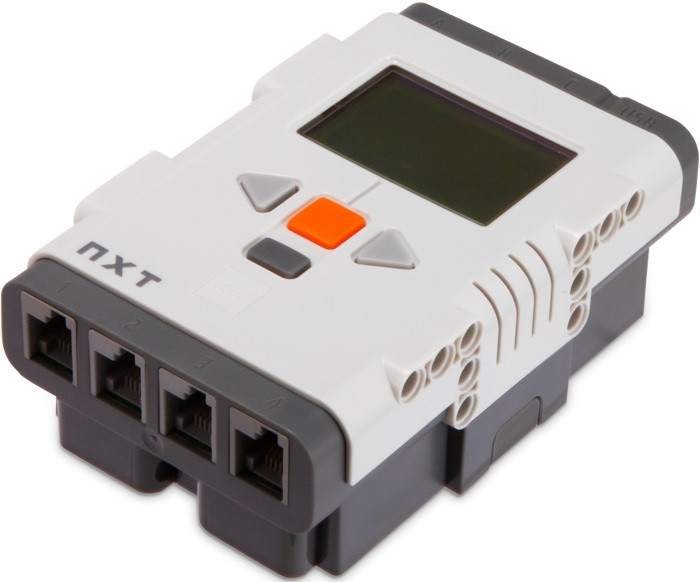
\includegraphics[width=4cm]{images/techAnalysis/LegoNXT2.jpg}
  \caption{LEGO MINDSTORMS NXT 2.0 brick \cite{BrickOWl-figure-NXT2}}\label{fig:sssec:LEGONXT2-NXT2}
\end{figure}
Where the EV3 brick is the key component in the LEGO MINDSTORMS universe, the predecessor to the EV3 brick is the NXT 2.0 brick.
Compared to the EV3, the NXT 2.0 is more limited in regards to its hardware specifications, as it only has a 48MHz 32-bit ARM7 processor with 64KB of RAM and 256KB flash memory, which can not be extended with a SDHC card.
The brick has four sensor ports and three motor ports, which is one motor port less than the EV3.
These are attached to the brick though RJ12 cables, like the EV3 \cite{LEGO_ev3_nodate}.
The NXT 2.0 can communicate through USB cable or Bluetooth, but not WIFI, allows for controlling through its physically buttons on the brick, and information can be seen on the 100x64 pixel built-in display.
Like the EV3 the NXT 2.0 brick also have speakers, but the sound quality is not as good.
Like the EV3, the NXT 2.0 can be powered by power supply or by batteries which can either be six AA batteries or a rechargeable battery pack. \cite{montes_real-time_2019, lego_mindstorms_2009}
